\documentclass[amsfonts, amssymb, aps, nofootinbib]{revtex4-2}
\usepackage[T1]{fontenc}
\usepackage{tgtermes}
\usepackage{amsmath}
\usepackage{empheq}
\usepackage{graphicx}
\usepackage{booktabs}
\usepackage[braket, qm]{qcircuit}
\usepackage{braket}
\usepackage{hyperref}
\usepackage{xcolor}
\usepackage{tikz}
\hypersetup{
	colorlinks   = true, %Colours links instead of ugly boxes
	urlcolor     = blue, %Colour for external hyperlinks
	linkcolor    = blue, %Colour of internal links
	citecolor   = red %Colour of citations
}

\newcommand{\cpflow}{\textit{cpflow }}
\newcommand{\static}{\textit{static }}
\newcommand{\adaptive}{\textit{adaptive }}
\newcommand{\CZ}{$CZ$}
\newcommand{\CP}{$CP$}
\newcommand{\T}{$T$}
\newcommand{\tgate}[1]{\textcolor{red}{#1}}
\newcommand{\cx}[1]{C${}^{#1}$X}
\begin{document}
\title{Optimal variational synthesis of small-scale quantum circuits.}
\begin{abstract}
	We consider the problem of variational unitary synthesis. 
\end{abstract}
\maketitle	
\tableofcontents
\section{Introduction}
\begin{itemize}
	\item Compilation -- translate from high-level algorithm to hardware instructions
	\item Relation to hardware efficient variational algorithms
	
\end{itemize}

\begin{align}
TLB(n) = \frac14\left(4^n-3n-1\right) \ . \label{TLB}
\end{align}

\begin{align}
d(U,V)=1-\frac1{4^n}|\operatorname{Tr}{U^\dagger V}|^2 \ . \label{d hst}
\end{align}

\begin{align}
\scalebox{1.0}{
	\Qcircuit @C=1.0em @R=0.8em @!R {
	 & \ctrl{2} & \qw \\
		CZ=\qquad\qquad& &\qquad\qquad\qquad\qquad\quad	= {\begin{pmatrix}1&0&0&0\\0&1&0&0\\0&0&1&0\\0&0&0&-1\end{pmatrix}}		\\
		& \control\qw & \qw \\
		\\ }} \label{def CZ}
	\\
\scalebox{1.0}{
	\Qcircuit @C=1.0em @R=0.8em @!R { \\
		& \ctrl{2} & \dstick{\hspace{2.0em}\mathrm{P}\,(\mathrm{a})} \qw \\
		CP(a)=\qquad\qquad& &\qquad\qquad\qquad\qquad\qquad\qquad\qquad	= {\begin{pmatrix}1&0&0&0\\0&1&0&0\\0&0&1&0\\0&0&0&e^{i\pi a}\end{pmatrix}}\\
		& \control \qw & \qw\\
		\\ }} \label{def CP}
\end{align}

\subsection{Template circuits}
Following \cite{Madden2021, Rakyta2021} we will construct the template circuits out of two-qubit blocks repeated in a regular manner. The two types of entangling blocks we will use are CZ- and CP-blocks depicted at fig.\ref{fig blocks}. They only differ by the type of the entangling gates used. 
\begin{figure}[h!]
\centering
\scalebox{1.0}{(a)
	\Qcircuit @C=1.0em @R=0.2em @!R { \\
		& \ctrl{1} & \gate{\mathrm{R_X}\,(\mathrm{a_0})} & \gate{\mathrm{R_Z}\,(\mathrm{a_1})} & \qw & \qw\\
		& \control\qw & \gate{\mathrm{R_X}\,(\mathrm{a_2})} & \gate{\mathrm{R_Z}\,(\mathrm{a_3})} & \qw & \qw\\
		\\ }}\qquad\qquad\qquad
\scalebox{1.0}{(b)
	\Qcircuit @C=1.0em @R=0.2em @!R { \\
		& \ctrl{1} & \dstick{\hspace{2.0em}\mathrm{P}\,(\mathrm{a_5})} \qw & \qw & \qw & \gate{\mathrm{R_X}\,(\mathrm{a_0})} & \gate{\mathrm{R_Z}\,(\mathrm{a_1})} & \qw & \qw\\
		& \control \qw & \qw & \qw & \qw & \gate{\mathrm{R_X}\,(\mathrm{a_2})} & \gate{\mathrm{R_Z}\,(\mathrm{a_3})} & \qw & \qw\\
		\\ }}
\caption{(a) CZ block (b) CP block.}
\label{fig blocks}
\end{figure}

The blocks are further arranged in sequences we refer to as \textit{layers}. In principle layers can can be arbitrary, but we will usually identify layers with coupling maps of the target topology. For example fig.\ref{fig layers} shows layers for the fully connected and 1D topology.
\begin{figure}[h!]
\centering
\scalebox{1.0}{(a) Connected layer
	\Qcircuit @C=1.0em @R=0.8em @!R { \\
		 & \ctrl{1} & \ctrl{2} & \ctrl{3} & \qw & \qw & \qw & \qw \\
		& \control\qw & \qw & \qw & \ctrl{1} & \ctrl{2} & \qw & \qw \\
		& \qw & \control\qw & \qw & \control\qw & \qw & \ctrl{1} & \qw\\
		& \qw & \qw & \control\qw & \qw & \control\qw & \control\qw & \qw \\
		\\ }}\qquad\qquad\qquad
\scalebox{1.0}{ (b) Chain layer
	\Qcircuit @C=1.0em @R=0.8em @!R { \\
		& \ctrl{1} & \qw & \qw & \qw\\
		& \control\qw & \ctrl{1} & \qw & \qw\\
		& \qw & \control\qw & \ctrl{1} & \qw\\
		& \qw & \qw & \control\qw & \qw\\
		\\ }}
\caption{(a) 4q connected layer (b) 4q chain layer. Here CZ gates are only meant to specify locations of 2q blocks, not their content. }
\label{fig layers}
\end{figure}

Finally, to fully specify the template one must provide the total \textit{number of 2q gates}. Layers are repeated until the specified number of 2q gates is reached, the last layer is truncated if needed. 
For illustration, fig.\ref{fig template example} depicts the full template circuit corresponding to 3q chain layer of CZ-blocks with 5 2q gates in total.

\begin{figure}[h!]
\scalebox{0.7}{
	\Qcircuit @C=1.0em @R=0.2em @!R { \\
		& \gate{\mathrm{R_Z}\,(\mathrm{a_{0}})} & \gate{\mathrm{R_X}\,(\mathrm{a_{1}})} & \gate{\mathrm{R_Z}\,(\mathrm{a_{2}})} & \ctrl{1} & \gate{\mathrm{R_X}\,(\mathrm{a_{9}})} & \gate{\mathrm{R_Z}\,(\mathrm{a_{10}})} & \qw & \qw & \qw & \ctrl{1} & \gate{\mathrm{R_X}\,(\mathrm{a_{17}})} & \gate{\mathrm{R_Z}\,(\mathrm{a_{18}})} & \qw & \qw & \qw & \ctrl{1} & \gate{\mathrm{R_X}\,(\mathrm{a_{25}})} & \gate{\mathrm{R_Z}\,(\mathrm{a_{26}})} & \qw & \qw\\
		& \gate{\mathrm{R_Z}\,(\mathrm{a_{3}})} & \gate{\mathrm{R_X}\,(\mathrm{a_{4}})} & \gate{\mathrm{R_Z}\,(\mathrm{a_{5}})} & \control\qw & \gate{\mathrm{R_X}\,(\mathrm{a_{11}})} & \gate{\mathrm{R_Z}\,(\mathrm{a_{12}})} & \ctrl{1} & \gate{\mathrm{R_X}\,(\mathrm{a_{13}})} & \gate{\mathrm{R_Z}\,(\mathrm{a_{14}})} & \control\qw & \gate{\mathrm{R_X}\,(\mathrm{a_{19}})} & \gate{\mathrm{R_Z}\,(\mathrm{a_{20}})} & \ctrl{1} & \gate{\mathrm{R_X}\,(\mathrm{a_{21}})} & \gate{\mathrm{R_Z}\,(\mathrm{a_{22}})} & \control\qw & \gate{\mathrm{R_X}\,(\mathrm{a_{27}})} & \gate{\mathrm{R_Z}\,(\mathrm{a_{28}})} & \qw & \qw\\
		& \gate{\mathrm{R_Z}\,(\mathrm{a_{6}})} & \gate{\mathrm{R_X}\,(\mathrm{a_{7}})} & \gate{\mathrm{R_Z}\,(\mathrm{a_{8}})} & \qw & \qw & \qw & \control\qw & \gate{\mathrm{R_X}\,(\mathrm{a_{15}})} & \gate{\mathrm{R_Z}\,(\mathrm{a_{16}})} & \qw & \qw & \qw & \control\qw & \gate{\mathrm{R_X}\,(\mathrm{a_{23}})} & \gate{\mathrm{R_Z}\,(\mathrm{a_{24}})} & \qw & \qw & \qw & \qw & \qw\\
		\\ }}
\caption{Template circuit $U(chain, CZ, 5)$.}
\label{fig template example}
\end{figure}



\section{Challenges to variational synthesis}
\subsection{Generally}
\begin{itemize}
	\item Discrete search over architectures 
	\item Continuous optimization
	\item Overview of existing software: QFAST, QSearch, SQUANDER
\end{itemize}
In variational algorithms: barren plateaus and local minimums. We: only local minimums.
\subsection{Focus on local minimums}



We will quantify the challenges associated with local minimums by the empirical success ratio
\begin{align}
	SR=\frac{M}{N} \ ,
\end{align}
where $N$ is the total number of times the optimization procedure is performed starting with different random initial conditions and $M$ is the number of times a global minimum is reached. 

For example, let $U(a)$ be the unitary matrix of the template circuit from fig.\ref{fig template example} and $a^*$ be some particular choice of angles. It is clear that the global minimum of the Hilbert-Schmidt distance \eqref{d hst} $d(U(a), U(a^*))$ is zero, but gradient-based optimization does not always reach it. For some choice of $a^*$ and out default optimizer specification (\ref) we find that the success ratio in this case is $SR=0.39$ from a 100 samples, which implies that roughly half of the times optimization gets stuck in a local minimum. 

We now extend this simple numerical experiment. Fig.\ref{fig local minumums} charts the success ratios for 3q and 4q circuits as a function of the number of gates. The basic procedure is the same with several additions. First, we used templates with fully connected layers (see fig.\ref{fig layers}) extended to the required number of 2q gates. For each number of 2q gates we take 10 different parameter assignments $a^*$ and compute success ratios for each of them using 2000 initial conditions. Blue markers represent mean success ratios averaged over 10 target circuits, while error bars quantify the standard deviation. Absence of blue markers implies that the the empirical success ratio was zero from 2000 samples. For 4q circuits datapoints were collected only every third integer.

There are several remarkable features that deserve highlighting. First, the success ratio drops very quickly as the 2q gate count increases, reaching values below $10^{-3}$ at 11 CZ gates for 3q circuits and 18 CZ gates fro 4q circuits. Next, perhaps surprisingly, the success ratio rises back and gets close to unity as the number of CZ gates approaches the theoretical lower bound \eqref{TLB} in agreement with the empirical evidence found in the literature \cite{Madden2021, Rakyta2021, Kiani2020}. A plausible explanation for this fact \cite{Ge2022} is that when the template is sufficiently expressive, optimization w.r.t. parameters becomes essentially the same as optimization over the unitary matrices themselves. At the same time, cost functions typically considered in quantum computing are simple, often linear or quadratic functions of the unitary matrix elements and hence are not prone to local minimums. Finally, although there is a certain spread of success ratio across different template instances, dependence on 2q gate count sets the dominating trend.

This suggests that success ratio is mostly a function of the template, not of the target. To confirm this  intuition  we carried out additional experiments using random unitaries $V$ instead of template instances as targets. The difficulty here is that the true value of the global minimum of $d(U(a), V)$ is not known, but the presence of local minimums is still manifest. We modify definition of the success ratio in this case, by counting as successful all optimization runs that approached sufficiently closely the lowest value of $d$ across all runs for a given unitary. Note that with this modified definition the success ratio can never be zero (because there is always at least a single run with the lowest value). We see that in the regime when success ratios for random instances are sufficiently high success ratios for random unitaries closely parallel, both in mean and in deviation. In the regions where success ratios for random instances are zero, success ratios for random unitaries are non-zero (they can not be by construction) but are sufficiently close to zero. We expect them to drop further if more samples are accounted for. Overall, our experiments strongly suggest that local minimums are mostly determined by the templates and not by targets.

Of course, success ratio is not only a function of the loss landscape but also of the optimization algorithm. Mathematically the problem of variational synthesis is very similar to the classical optimization subroutines encountered in variational algorithms \cite{}, especially in the subclass referred to as  hardware-efficient \cite{Kandala2017}\cite{}. The problem of local minimums is well appreciated in the relevant literature. It was shown to be NP-hard in the worst case \cite{Bittel2021}. On the heuristic side there are a number of proposals to alleviate the problem \cite{Wierichs2020, Rivera-Dean2021, ?} but in our experiments none performed sufficiently better than simple ADAM\cite{adam}-based optimization to justify additional computational resources that are typically required.

\begin{figure}
\includegraphics[width=0.4\textwidth]{figures/3q_success_chart}
\includegraphics[width=0.4\textwidth]{figures/4q_success_chart}
\caption{Local minimums as a function of circuit complexity. Datapoints for random unitaries are advanced by a half unit along $x$ axis for clarity.}
\label{fig local minumums}
\end{figure}

\begin{itemize}
	\item 3q and 4q charts.
	\item Separately marked Toffoli gates
\end{itemize}
\section{The CPFlow algorithm}
\subsection{Motivation and overview}
In the context of variational synthesis results of the previous section suggest that solving the continuous optimization problem may be just as difficult as solving the discrete architecture search: even if the structure of the template is a perfect match for the target unitary, finding the suitable angles may be very challenging. In the absence of an efficient way to solve the latter problem in our approach we choose the brute force route of trying many initial conditions. A second main idea of our approach is to reformulate the discrete architecture search as a continuous problem as well \footnote{While this work was in preparation similar idea was independently introduced in \cite{Rakyta2022}.}. For illustration, consider the circuit at fig.\ref{fig cp example}.
\begin{figure}[h!]
\scalebox{0.7}{
	\Qcircuit @C=1.0em @R=0.2em @!R { \\
		 & \gate{\mathrm{R_Z}\,(\mathrm{a_{0}})} & \gate{\mathrm{R_X}\,(\mathrm{a_{1}})} & \gate{\mathrm{R_Z}\,(\mathrm{a_{2}})} & \ctrl{1} & \dstick{\hspace{2.0em}\mathrm{P}\,(\mathrm{a_{13}})} \qw & \qw & \qw & \gate{\mathrm{R_X}\,(\mathrm{a_{9}})} & \gate{\mathrm{R_Z}\,(\mathrm{a_{10}})} & \ctrl{2} & \qw & \qw & \qw & \gate{\mathrm{R_X}\,(\mathrm{a_{14}})} & \gate{\mathrm{R_Z}\,(\mathrm{a_{15}})} & \qw & \qw & \qw & \qw & \qw & \qw & \qw & \qw\\
		& \gate{\mathrm{R_Z}\,(\mathrm{a_{3}})} & \gate{\mathrm{R_X}\,(\mathrm{a_{4}})} & \gate{\mathrm{R_Z}\,(\mathrm{a_{5}})} & \control \qw & \qw & \qw & \qw & \gate{\mathrm{R_X}\,(\mathrm{a_{11}})} & \gate{\mathrm{R_Z}\,(\mathrm{a_{12}})} & \qw & \dstick{\hspace{2.0em}\mathrm{P}\,(\mathrm{a_{18}})} \qw & \qw & \qw & \qw & \qw & \ctrl{1} & \dstick{\hspace{2.0em}\mathrm{P}\,(\mathrm{a_{23}})} \qw & \qw & \qw & \gate{\mathrm{R_X}\,(\mathrm{a_{19}})} & \gate{\mathrm{R_Z}\,(\mathrm{a_{20}})} & \qw & \qw\\
		& \gate{\mathrm{R_Z}\,(\mathrm{a_{6}})} & \gate{\mathrm{R_X}\,(\mathrm{a_{7}})} & \gate{\mathrm{R_Z}\,(\mathrm{a_{8}})} & \qw & \qw & \qw & \qw & \qw & \qw & \control \qw & \qw & \qw & \qw & \gate{\mathrm{R_X}\,(\mathrm{a_{16}})} & \gate{\mathrm{R_Z}\,(\mathrm{a_{17}})} & \control \qw & \qw & \qw & \qw & \gate{\mathrm{R_X}\,(\mathrm{a_{21}})} & \gate{\mathrm{R_Z}\,(\mathrm{a_{22}})} & \qw & \qw\\
		\\ }}
\caption{Exemplary CP template. Draw possible architechres \ref{}}
\label{fig cp example}
\end{figure}

Here 2q gates are controlled phase (CP) gates \eqref{def CP} which interpolate between the identity gate $CP(0)=\mathbb{I}$ and the $CZ$ \eqref{def CZ} gate $CP(\pi)=CZ$. For generic values of the angle the $CP(a)$ gate can be decomposed into 2 $CZ$ gates \ref{}. Therefore, different values of parameters in $CP$ gates in the template \eqref{fig cp example} effectively capture several different templates with $CZ$ 2q gates and training templates with $CP$-blocks can encompass both the architecture search and the tuning of continuous parameters, moreover performed in a coherent manner.


We can anticipate, however, that training $CP$ templates to minimize the Hilbert-Schmidt distance to the target unitary directly will result in most $CP$ gates having generic angles and hence effectively double the $CZ$ count of the original template. To address this issue we introduce additional \textit{penalty term} to the cost function that is intended to drive all $CP$ angles either to $0$ or to $\pi$. The shape of the penalty function that we use is presented at fig.\ref{fig penalty}.
\begin{figure}[h!]
\includegraphics[width=0.4\textwidth]{figures/penalty}
\caption{Penalty function for angles of the $CP$-gates. For clarity of the figure, width of plateaus near $0,\frac12\pi, \frac32\pi, 2\pi$} is twice the value used in numerical experiments.
\label{fig penalty}
\end{figure}

This penalty is intended to drive all $CP$-angles during optimization to either $0$ or $\pi$ and hence to reduce the $CZ$-count of the resulting circuit. For numerical stability small plateaus are added near values $0,\pi$ and also $\frac12\pi, \frac32\pi$  (empirically we find that $CP$ angles are often equilibrate near these values too).

\subsection{Procedure}
We formulate the general synthesis problem as follows. Let $L(U)$ be the loss function to be minimized with unitary as the argument. For unitary synthesis $L(U)$ may be any measure of fidelity to the target unitary $V$, for example $L(U)=D(U, V)$. For state preparation we can choose $L(U) = \Big|\braket{\psi|U|0}\Big|^2$ where $\ket{\psi}$ is the target state and $\ket{0}$ is the usual reference state, etc. The goal is to find a unitary $U^k_{CZ}(a)$ such that $L(U^k_{CZ}(a))$ is sufficiently close to the global minimum of $L(U)$ and at the same time the number $k$ of 2q gates in $U^k_{CZ}$ is as small as possible. 

The loss function directly addressed by CPFlow is given by
\begin{align}
\mathcal{L}(a)=L(U^k_{CP}(a))+r\sum_{a_i\in CP} R(a_i) \label{CP loss}
\end{align}
The first term is simply the value of the loss function at the given unitary. The second term is the regularization term summing the $CP$-penalties for all $CP$-angles in the circuit. The number of 2q gates $k$ and the overall regularization weight $r$ are two of the most important hyperparameters of the model.

Three main stages of the algorithm are as follows.

\begin{enumerate}
\item \textit{\textbf{ Raw sampling.}} Loss function \eqref{CP loss} is minimized starting from many initial conditions. Both the $CP$-angles and angles of 1q gates are selected uniformly and independently at random\footnote{Distribution of $CP$ angles could be changed.}. 
\item \textit{\textbf{Selecting prospective results.}} Results of the first step are selected based on two criteria (i) the original loss function $L(U^k_{CP}(a^*))$ must be below a given threshold (typically we use $10^{-4}$) and (ii) the number of gates $\sum_{a_i\in CP}G(a_i)$ is below a specified value. Condition (i) means we only accept circuits that are close enough to the global minimum while (ii) filters out decompositions with too high $CZ$ count.
\item \textit{\textbf{Verification.}} Circuits selected at the previous step are first projected from $CP$ to $CZ$ circuits $U_{CP}^k(a)\to U_{CZ}^{k'}(a')$ by rounding off values of $CP$ gates that are sufficiently close to $0$ or $2\pi$ and substituting other $CP$ gates with their 2-CZ decompositions. 1q angles $a'$ are mostly inherited from $a$ except when a decomposition procedure was used. Next, the loss function $L(U_{CZ}^{k'}(a)$ (without the regularization term) is optimized starting from initial angles $a=a'$. The verification is considered successful if the projected $CZ$ circuit reaches a more stringent loss threshold (typically we use $10^{-6}$).
\end{enumerate}

This scheme can be modified in many ways: by choosing a different regularization function, using non-uniform sampling of initial angles, altering details of the gradient based optimizer to name a few. We have mostly experimented with varying two hyperparameters that are evidently crucial, the number of $CP$ gates $k$ and the regularization weight $r$. Heuristically, we find that a reasonable number of $CP$ gates is about twice as much as the expected $CZ$-count of the optimal solution and the value of $r$ for loss functions normalized so that $0\le L(U) \le 1$ is of order $r=5\times 10^{-4}$. To make better choices of hyperparameters on a case by case basis we use Bayesian tuning algorithm provided by Hyperopt package \cite{hyperopt, ?}. Tuning of hyperparameters is significantly hindered by the fact that the loss function is stochastic. Taking sufficiently many samples to reliably estimate the quality of a hyperparameter configuration may cost too much computational resources, while not taking enough the acquired data too noisy to be useful. On the positive side the goal of the algorithm is not to find the best hyperparameters, but rather to find the best decompositions, which can occur (although less likely) for suboptimal hyperparameters as well. The routine including hyperparameter tuning can be summarized as follows.

\begin{enumerate}
\item \textit{\textbf{Defining the search space.}} Choose a distribution to draw $k$ and $r$ from. Typically we use uniform distribution for $k$ in some integer range and lognormal distribution for $r$ with mean around $5\times 10^{-4}$ and standard deviation $0.5$.
\item \textit{\textbf{Evaluating score function.}} Draw a sample $k, r$ from the hyperparmeter distribution according to the Hyperopt algorithm. Execute steps 1 and 2 from the basic routine. Any $CZ$-count is accepted at this stage, i.e. the results are only selected by the value of the original loss function $L(U_{CP}^k(a))$. Let $k_1, k_2,\dots$ be $CZ$ counts of all prospective results selected. We define the score function (reminiscent of the \textit{softmin}) by 
\begin{align}
-\log_2\frac{1}{N}\sum_{i}2^{-k_i}
\end{align}
where $N$ is the total number of raw samples. The minimum of this function is $k_0$, the $CZ$-count of the best possible decomposition. It can be reached if all raw samples reached the threshold fidelity and have the optimal count $k_0$ when projected to $CZ$-circuits. The maximum is $+\infty$ when none of the raw samples passed the fidelity threshold.
\item \textit{\textbf{Verifying best decompositions.}} At the previous stage all prospective decompositions are not verified as the verification process is time-consuming is should not significantly alter the score estimation (some of the decompositions may fail to pass the verification, but this is rare). However, if there are prospective decompositions that improve on the current best they are verified and if accepted, the current best is replaced.

\item \textit{\textbf{Repeat.}} Repeat steps 2 and 3 until either the maximum number of score evaluations is reached or a decomposition with the desired number of gates is found.
\end{enumerate}
\subsection{Technical details}
The \textit{static} routine implemented in \cpflow uses the following default specifications (all could be customized by the user). At the raw sampling stage the optimization of the loss function \eqref{CP loss} is performed using ADAM\cite{} optimizer with learning rate $0.1$ and 2000 iterations. At the selection stage for each sample the best configuration of angles $a^*$ is chosen corresponding to the minimum of the regularized loss function \eqref{CP loss} across all iterations. If the primary loss function $L(U_{CP}^k(a^*))$ is below $10^{-4}$ threshold and the $CP$ circuit is projected to the $CZ$ circuit $U_{CP}^k(a^*)\to U_{CZ}^{k'}(a')$. Projection is performed as follows. $CP$-gates with angles lying withing the threshold distance (0.2 by default) away from $0$ or $\pi$ are replaced by identity and $CZ$ gates respectively.  $CP$-gates that were not replaced at the previous stage are decomposed into 2-$CZ$ decomposition using standard methods. If the 2q gate count $k'$ of the resulting $CZ$-circuit is within the accepted range the circuit is deemed prospective. At the verification stage the original loss function $L(U_{CZ}^{k'}(a))$ is further optimized with the ADAM optimizer, possibly with a smaller learning rate (0.01) and for larger number of iterations (5000). Importantly, the new optimization starts with the initial angles $a'$ obtained after projecting the $CP$ circuit. If the new optimization pass reaches a more stringent threshold ($10^{-6}$ by default) the verification is considered successful and the resulting circuit is added to the collection of decompositions.



\begin{itemize}
	\item Better than random search
	\item Exact synthesis
\end{itemize}
\section{Synthesis of Toffoli gates}
Toffoli gates are among the most essential building blocks for a great variety of quantum algorithms \cite{}. The basic Toffoli gate, also known as the Controlled-Controlled-NOT or the CCX gate is depicted as follows
\begin{align}
\scalebox{1.0}{
	\Qcircuit @C=1.0em @R=0.2em @!R { \\
		&&&&&\qw&\ctrl{1}&\qw&\qw&\qquad{ }\qquad&& \qw & \ctrl{1} & \qw & \qw \\
		&CCX&&\qquad&  =\qquad&\qw&\ctrl{1}&\qw&\qw&\qquad=\qquad&	& \qw & \ctrl{1} & \qw & \qw \\
		&&&&&\qw&\targ&\qw&\qw&\qquad{ }\qquad& & \gate{\mathrm{H}} & \control\qw & \gate{\mathrm{H}} & \qw\\
		\\ }}
\end{align}
The right diagram represents the Toffoli gate as the $CCZ$ gate conjugated by the two Hadamard gates ($HZH=X$). The $CCZ$ gate itself is represented by a diagonal matrix $CCZ=\operatorname{diag}(1,1,1,1,1,1,1,-1)$ and is symmetric with respect to all qubits. Therefore, up to a conjugation by 1q gates the Toffoli gates (C${}^2$X as well as C${}^{n}$X) are also symmetric wrt all qubits. This implies that even if the symmetry between the qubits is broken by e.g. a non-trivial topology, the choice of the target qubit is not relevant for the synthesis problem.

Large multi-controlled Toffoli gates can be built recursively from the smaller ones \ref{}, hence optimization of the small-size Toffoli gates can be propagated to the large multi-controlled gates required in useful quantum algorithms. 

\subsection{Toffoli 3}
The basic Toffoli gate can be decomposed into 6 $CZ$ gates on the fully connected topology or 8 $CZ$ gates on the chain topology. Using the \cpflow we were able to find many inequivalent decompositions with these optimal \CZ-counts. First, we ran the \textit{adaptive} routine for a 100 score evaluations to identify the best hyperparameters in each case. Results are reported at fig.\ref{fig trials}. Best hyperparameters for each topology are shown in tab.\ref{tab toff3}. Note that at this stage decompositions with the optimal \CZ-count have already been found, but it is instructive to further analyze the performance of the algorithm and generate more decompositions.

To this end we ran the \static routine with optimal hyperparameters and 100 samples for each topology. Third column in tab.\ref{tab toff3} states how many of the initial conditions led to the decompositions with the optimal \CZ-count. For connected topology this is roughly $50\%$, while for chain topology about $10\%$. These figures are to be compared with the success ratios at the respective gate counts \ref{fig local minumums}, which are of order $15\%$ and $3\%$ respectively. The remarkable conclusion is that (at least in this simple example) out strategy our coherent learning of the architecture together with continuous parameters seems to be unreasonably efficient. With the best hyperparameters the frequency of finding \CZ-count optimal decompositions is greater than the corresponding success ratios.

Let conclude the illustration of the algorithm at work with the following observation. If the regularization weight $r$ is large enough, the regularization term in \eqref{CP loss} effectively captures each of the \CP-angles at the local minimum (0 or $\pi$) that it was originally sampled near. This is similar to ...


\begin{figure}
	Connected topology
	\scalebox{0.7}{
	\Qcircuit @C=1.0em @R=0.4em @!R { \\
	& \qw & \qw & \ctrl{1} & \gate{\mathrm{X}\,(\mathrm{\pi})} & \qw & \qw & \qw & \qw & \ctrl{1} & \qw & \ctrl{2} & \gate{\mathrm{Z}\,(\mathrm{-\pi})} & \gate{\mathrm{X}\,(\mathrm{\pi})} & \ctrl{2} & \gate{\tgate{\mathrm{Z}\,(\mathrm{\frac{\pi}{4}})}} & \qw & \qw & \qw & \qw & \qw & \qw & \qw\\
	& \gate{\mathrm{Z}\,(\mathrm{-\pi})} & \gate{\mathrm{X}\,(\mathrm{\frac{\pi}{2}})} & \control\qw & \gate{\mathrm{Z}\,(\mathrm{\frac{-\pi}{2}})} & \gate{\tgate{\mathrm{X}\,(\mathrm{\frac{\pi}{4}})}} & \ctrl{1} & \gate{\mathrm{Z}\,(\mathrm{-\pi})} & \gate{\tgate{\mathrm{X}\,(\mathrm{\frac{3\pi}{4}})}} & \control\qw & \gate{\tgate{\mathrm{X}\,(\mathrm{\frac{3\pi}{4}})}} & \qw & \qw & \qw & \qw & \qw & \qw & \ctrl{1} & \gate{\mathrm{Z}\,(\mathrm{\frac{\pi}{2}})} & \gate{\mathrm{X}\,(\mathrm{\frac{\pi}{2}})} & \gate{\tgate{\mathrm{Z}\,(\mathrm{\frac{\pi}{4}})}} & \qw & \qw\\
	& \gate{\mathrm{Z}\,(\mathrm{\frac{-\pi}{2}})} & \gate{\mathrm{X}\,(\mathrm{\frac{\pi}{2}})} & \qw & \qw & \qw & \control\qw & \gate{\mathrm{X}\,(\mathrm{\frac{\pi}{2}})} & \qw & \qw & \qw & \control\qw & \gate{\mathrm{Z}\,(\mathrm{\frac{-\pi}{2}})} & \gate{\tgate{\mathrm{X}\,(\mathrm{\frac{\pi}{4}})}} & \control\qw & \gate{\mathrm{Z}\,(\mathrm{\frac{-\pi}{2}})} & \gate{\mathrm{X}\,(\mathrm{\frac{\pi}{2}})} & \control\qw & \gate{\tgate{\mathrm{Z}\,(\mathrm{\frac{\pi}{4}}})} & \gate{\mathrm{X}\,(\mathrm{\frac{\pi}{2}})} & \gate{\mathrm{Z}\,(\mathrm{\frac{\pi}{2}})} & \qw & \qw\\
	\\ }}\\
Chain topology
\scalebox{0.65}{
	\Qcircuit @C=1.0em @R=0.2em @!R { \\
		& \gate{\mathrm{Z}\,(\mathrm{\frac{\pi}{2}})} & \gate{\mathrm{X}\,(\mathrm{\pi})} & \qw & \qw & \ctrl{1} & \gate{\mathrm{Z}\,(\mathrm{-\pi})} & \gate{\mathrm{X}\,(\mathrm{\pi})} & \qw & \ctrl{1} & \gate{\mathrm{Z}\,(\mathrm{-\pi})} & \gate{\mathrm{X}\,(\mathrm{\pi})} & \qw & \qw & \qw & \qw & \qw & \ctrl{1} & \gate{\mathrm{Z}\,(\mathrm{-\pi})} & \gate{\mathrm{X}\,(\mathrm{\pi})} & \gate{\tgate{\mathrm{Z}\,(\mathrm{\frac{5\pi}{4}})}} & \qw & \qw & \qw & \qw & \qw\\
		& \gate{\mathrm{X}\,(\mathrm{\frac{\pi}{2}})} & \ctrl{1} & \gate{\mathrm{Z}\,(\mathrm{-\pi})} & \gate{\mathrm{X}\,(\mathrm{\frac{\pi}{2}})} & \control\qw & \gate{\mathrm{X}\,(\mathrm{\frac{\pi}{2}})} & \ctrl{1} & \gate{\tgate{\mathrm{X}\,(\mathrm{\frac{3\pi}{4}})}} & \control\qw & \gate{\mathrm{Z}\,(\mathrm{\frac{-\pi}{2}})} & \gate{\mathrm{X}\,(\mathrm{\frac{\pi}{2}})} & \ctrl{1} & \gate{\tgate{\mathrm{Z}\,(\mathrm{\frac{-3\pi}{4}})}} & \gate{\mathrm{X}\,(\mathrm{\frac{\pi}{2}})} & \ctrl{1} & \gate{\mathrm{X}\,(\mathrm{\frac{\pi}{2}})} & \control\qw & \gate{\mathrm{Z}\,(\mathrm{\frac{-\pi}{2}})} & \gate{\mathrm{X}\,(\mathrm{\frac{\pi}{2}})} & \ctrl{1} & \gate{\mathrm{Z}\,(\mathrm{\frac{-\pi}{2}})} & \gate{\mathrm{X}\,(\mathrm{\frac{\pi}{2}})} & \gate{\tgate{\mathrm{Z}\,(\mathrm{\frac{\pi}{4}})}} & \qw & \qw\\
		& \qw & \control\qw & \gate{\mathrm{Z}\,(\mathrm{\pi})} & \gate{\mathrm{X}\,(\mathrm{\frac{\pi}{2}})} & \qw & \qw & \control\qw & \gate{\mathrm{Z}\,(\mathrm{-\pi})} & \gate{\tgate{\mathrm{X}\,(\mathrm{\frac{3\pi}{4}})}} & \qw & \qw & \control\qw & \gate{\tgate{\mathrm{X}\,(\mathrm{\frac{3\pi}{4}})}} & \qw & \control\qw & \gate{\mathrm{Z}\,(\mathrm{\frac{-\pi}{2}})} & \gate{\mathrm{X}\,(\mathrm{\frac{\pi}{2}})} & \qw & \qw & \control\qw & \gate{\mathrm{Z}\,(\mathrm{-\pi})} & \gate{\tgate{\mathrm{X}\,(\mathrm{\frac{3\pi}{4}})}} & \gate{\mathrm{Z}\,(\mathrm{\pi})} & \qw & \qw\\
		\\ }}
\label{fig toff3}
\caption{Decompositions of Toffoli 3 gate that are likely to be optimal with respect to all four metrics: \CZ-depth, \CZ-count, \T-depth, \T-count. Non-Clifford gates are highlighted.}
\end{figure}

\begin{figure}
\includegraphics[scale=0.5]{figures/toff3_trials_conn}
\includegraphics[scale=0.5]{figures/toff3_trials_chain}
\caption{Visualization of hyperparameter optimization in synthesis of Toffoli gate on connected (left panel) and chain (right panel) topologies. Red crosses corresponds to infinite score value and imply that no valid decompositions were found at these points. Gold star marks the best hyperparameter configuration.}
\label{fig trials}	
\end{figure}
\begin{table}[]
	\begin{tabular}{@{}ccccc@{}}
		\toprule
		& best k & best r              & Optimal decompositions &  \\ \midrule
		Connected & 6      & $0.82\times10^{-3}$ & 49/100                 &  \\
		Chain     & 14     & $0.96\times10^{-3}$ & 8/100                  &  \\ \bottomrule
	\end{tabular}
\label{tab toff3}
\end{table}
\subsection{Toffoli 4}
Variational synthesis of the C${}^{3}$X gate on various 4q topologies has been recently addressed in \cite{Nakanishi2021}. Using \cpflow we were able to reproduce all results presented there and achieve a minor improvement for the star-shaped topology, see table \ref{tab toff4}.

\begin{table}[]
	\begin{tabular}{@{}cccccc@{}}
		\toprule
		Topology
		&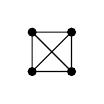
\begin{tikzpicture}[scale=0.5]
		\draw[fill] (0,0) circle [radius=0.1];
		\draw[fill] (0,1) circle [radius=0.1];
		\draw[fill] (1,0) circle [radius=0.1];
		\draw[fill] (1,1) circle [radius=0.1];
		
		\draw (0,0) -- (1, 0) -- (1, 0) -- (1, 1) -- (0, 1) -- (0, 0) -- (1, 1);
		\draw (1, 0) -- (0, 1);
		\end{tikzpicture} 
		&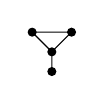
\begin{tikzpicture}[scale=0.5]
		\draw[fill] (0.5,0) circle [radius=0.1];
		\draw[fill] (0.5,0.5) circle [radius=0.1];
		\draw[fill] (0,1) circle [radius=0.1];
		\draw[fill] (1,1) circle [radius=0.1];
		
		\draw (0.5, 0) -- (0.5, 0.5) -- (1, 1) -- (0, 1) -- (0.5, 0.5);
		\end{tikzpicture}
		&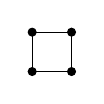
\begin{tikzpicture}[scale=0.5]
		\draw[fill] (0,0) circle [radius=0.1];
		\draw[fill] (0,1) circle [radius=0.1];
		\draw[fill] (1,0) circle [radius=0.1];
		\draw[fill] (1,1) circle [radius=0.1];
		
		\draw (0,0) -- (1, 0) -- (1, 1) -- (0, 1) -- (0, 0);
		\end{tikzpicture}  
		&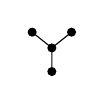
\begin{tikzpicture}[scale=0.5]
		\draw[fill] (0.5,0) circle [radius=0.1];
		\draw[fill] (0.5,0.6) circle [radius=0.1];
		\draw[fill] (0,1) circle [radius=0.1];
		\draw[fill] (1,1) circle [radius=0.1];
		
		\draw (0.5, 0) -- (0.5, 0.6) -- (1, 1);
		\draw (0.5, 0.6) -- (0, 1);
		\end{tikzpicture}    
		& 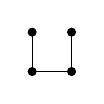
\begin{tikzpicture}[scale=0.5]
		\draw[fill] (0,0) circle [radius=0.1];
		\draw[fill] (0,1) circle [radius=0.1];
		\draw[fill] (1,0) circle [radius=0.1];
		\draw[fill] (1,1) circle [radius=0.1];
		
		\draw (0,1) -- (0, 0) -- (1, 0) -- (1, 1);
		\end{tikzpicture}   \\ \midrule
		CZ count & 14 (14)   & 14 (14) & 16 (16) & 16 (17) & 18 (18) \\
		CZ depth &           &         &         &         & \\ \bottomrule       
	\end{tabular}
\caption{Decompositions of 4q Toffoli gate on various topolgies}
\label{tab toff4}
\end{table}

\subsection{Toffoli 5}
To the best of our knowledge, the best decomposition of \cx{4}

\section{Benchmarks and results}
\subsection{Clifford+T from database}
\subsection{State prep for error correction}
\section{Synthesis of special gates}
\subsection{Toffoli 3 on chain up to SWAP}
\subsection{Toffoli 4 on all topologies including new record at T-shaped}
\subsection{Toffoli 5 already difficult, can be done separating into parts}

\bibliography{/home/idnm/Dropbox/hep/Sheets/library.bib, bibfile.bib}
\end{document}

\begin{figure}
	
	\centering{\text{Template circuit}}
	
	\scalebox{0.7}{
		\Qcircuit @C=1.0em @R=0.2em @!R { \\
			& \gate{\mathrm{R_Z}\,(\mathrm{a_{0}})} & \gate{\mathrm{R_X}\,(\mathrm{a_{1}})} & \gate{\mathrm{R_Z}\,(\mathrm{a_{2}})} & \ctrl{1} & \gate{\mathrm{R_X}\,(\mathrm{a_{9}})} & \gate{\mathrm{R_Z}\,(\mathrm{a_{10}})} & \ctrl{2} & \gate{\mathrm{R_X}\,(\mathrm{a_{13}})} & \gate{\mathrm{R_Z}\,(\mathrm{a_{14}})} & \qw & \qw & \qw & \ctrl{1} & \gate{\mathrm{R_X}\,(\mathrm{a_{21}})} & \gate{\mathrm{R_Z}\,(\mathrm{a_{22}})} & \qw & \qw\\
			& \gate{\mathrm{R_Z}\,(\mathrm{a_{3}})} & \gate{\mathrm{R_X}\,(\mathrm{a_{4}})} & \gate{\mathrm{R_Z}\,(\mathrm{a_{5}})} & \control\qw & \gate{\mathrm{R_X}\,(\mathrm{a_{11}})} & \gate{\mathrm{R_Z}\,(\mathrm{a_{12}})} & \qw & \qw & \qw & \ctrl{1} & \gate{\mathrm{R_X}\,(\mathrm{a_{17}})} & \gate{\mathrm{R_Z}\,(\mathrm{a_{18}})} & \control\qw & \gate{\mathrm{R_X}\,(\mathrm{a_{23}})} & \gate{\mathrm{R_Z}\,(\mathrm{a_{24}})} & \qw & \qw\\
			& \gate{\mathrm{R_Z}\,(\mathrm{a_{6}})} & \gate{\mathrm{R_X}\,(\mathrm{a_{7}})} & \gate{\mathrm{R_Z}\,(\mathrm{a_{8}})} & \qw & \qw & \qw & \control\qw & \gate{\mathrm{R_X}\,(\mathrm{a_{15}})} & \gate{\mathrm{R_Z}\,(\mathrm{a_{16}})} & \control\qw & \gate{\mathrm{R_X}\,(\mathrm{a_{19}})} & \gate{\mathrm{R_Z}\,(\mathrm{a_{20}})} & \qw & \qw & \qw & \qw & \qw\\
			\\ }}
	
	\centering{\text{Target circuit}}	
	
	\scalebox{0.7}{
		\Qcircuit @C=1.0em @R=0.2em @!R { \\
			& \gate{\mathrm{R_Z}\,(\mathrm{6.246})} & \gate{\mathrm{R_X}\,(\mathrm{0.5124})} & \gate{\mathrm{R_Z}\,(\mathrm{1.219})} & \ctrl{1} & \gate{\mathrm{R_X}\,(\mathrm{1.903})} & \gate{\mathrm{R_Z}\,(\mathrm{5.638})} & \ctrl{2} & \gate{\mathrm{R_X}\,(\mathrm{2.711})} & \gate{\mathrm{R_Z}\,(\mathrm{5.384})} & \qw & \qw & \qw & \ctrl{1} & \gate{\mathrm{R_X}\,(\mathrm{1.105})} & \gate{\mathrm{R_Z}\,(\mathrm{1.16})} & \qw & \qw\\
			& \gate{\mathrm{R_Z}\,(\mathrm{4.646})} & \gate{\mathrm{R_X}\,(\mathrm{2.216})} & \gate{\mathrm{R_Z}\,(\mathrm{1.714})} & \control\qw & \gate{\mathrm{R_X}\,(\mathrm{2.833})} & \gate{\mathrm{R_Z}\,(\mathrm{0.6454})} & \qw & \qw & \qw & \ctrl{1} & \gate{\mathrm{R_X}\,(\mathrm{2.812})} & \gate{\mathrm{R_Z}\,(\mathrm{2.779})} & \control\qw & \gate{\mathrm{R_X}\,(\mathrm{2.515})} & \gate{\mathrm{R_Z}\,(\mathrm{2.283})} & \qw & \qw\\
			& \gate{\mathrm{R_Z}\,(\mathrm{6.106})} & \gate{\mathrm{R_X}\,(\mathrm{2.695})} & \gate{\mathrm{R_Z}\,(\mathrm{1.408})} & \qw & \qw & \qw & \control\qw & \gate{\mathrm{R_X}\,(\mathrm{5.926})} & \gate{\mathrm{R_Z}\,(\mathrm{0.1336})} & \control\qw & \gate{\mathrm{R_X}\,(\mathrm{3.677})} & \gate{\mathrm{R_Z}\,(\mathrm{1.53})} & \qw & \qw & \qw & \qw & \qw\\
			\\ }}
	
	\caption{Exemplary template and target circuits.}	
	\label{fig SR circuits}
\end{figure}